\documentclass[usenames, dvipsnames, aspectratio = 169, 13pt]{beamer}

\usepackage{color}
% Typesetting
	\usepackage{amsfonts}
	\usepackage{amssymb}
	\usepackage{amsmath}

	\usepackage{subfig}

	\usepackage{graphicx}
    
    \usepackage{multicol}
    \usepackage{tikz}
    \usetikzlibrary{calc,intersections}
    
    \usepackage{dcolumn}
    
    \usepackage{accents}
    \usepackage{adjustbox}

% Bibliography
    % \usepackage[style=authoryear-comp,natbib=true,backend=biber]{biblatex}
    % \addbibresource{Bibliography.bib}
    % \usepackage{csquotes}
	\usepackage{natbib}
 	%\bibliographystyle{apalike}
 	\bibliographystyle{aer}
	
	\usepackage{bibunits}
	\defaultbibliography{Bibliography.bib}  
	%\defaultbibliographystyle{apalike}
	\defaultbibliographystyle{aer}

	
% Links
	\usepackage{hyperref}
	\hypersetup{
    colorlinks=true,
    linkcolor=black,
    filecolor=magenta,      
    urlcolor=blue,
    citecolor = black
}
	\usepackage{cleveref}

% Todonotes
	\usepackage[framemethod=tikz]{mdframed}
	\usepackage{todonotes}
	\presetkeys{todonotes}{color=black!5,inline}{} % noline

% Boxes
    \usepackage{tcolorbox}
    \newtcbox{\feedback}{nobeforeafter,colframe=black,colback=white,boxrule=0.5pt,arc=2pt,
      boxsep=0pt,left=2pt,right=2pt,top=2pt,bottom=2pt,tcbox raise base}
      
% Theorems
    \usepackage{amsthm}
     
    \newtheorem{thm}{Theorem}
    \newtheorem{asm}{Assumption}
    \newtheorem{con}{Conjecture}
    \newtheorem{prop}{Proposition}
    \newtheorem{lem}{Lemma}
    \newtheorem{cor}{Corollary}
    \newtheorem{rem}{Remark}
    \newtheorem{defn}{Definition}

%Packages and commands for column widths in tables
\usepackage{array}
\newcolumntype{L}[1]{>{\raggedright\let\newline\\\arraybackslash}m{#1}}
\newcolumntype{C}[1]{>{\centering\let\newline\\\arraybackslash\hspace{0pt}}m{#1}}
\newcolumntype{R}[1]{>{\raggedleft\let\newline\\\arraybackslash\hspace{0pt}}m{#1}}

%Turn off toolbar
\setbeamertemplate{navigation symbols}[default]
\beamertemplatenavigationsymbolsempty  


%Macro for wrapping text in underbrace
\usepackage{ragged2e}
\newlength\ubwidth
\newcommand\wrapunderbrace[2]{\settowidth\ubwidth{$#1$}\underbrace{#1}_{\parbox{\ubwidth}{\scriptsize\RaggedRight#2}}}


%This makes citations smaller
\makeatletter
\DeclareRobustCommand\citep
{\begingroup\footnotesize\NAT@swatrue\let\NAT@ctype\z@\NAT@partrue
    \@ifstar{\NAT@fulltrue\NAT@citetp}{\NAT@fullfalse\NAT@citetp}}
\makeatother
% Probability
\renewcommand{\P}{\mathop{}\!\textnormal{P}}
\newcommand{\E}{\mathop{}\!\textnormal{E}}
\newcommand{\sE}{\mathop{}\!\mathbb{E}}
\newcommand{\Cov}{\mathop{}\!\textnormal{Cov}}
\newcommand{\sCov}{\mathop{}\!\mathbb{C}\textnormal{ov}}
\newcommand{\Var}{\mathop{}\!\textnormal{Var}}
\newcommand{\sVar}{\mathop{}\!\mathbb{V}\textnormal{ar}}
\newcommand{\N}{\mathcal{N}}
\newcommand{\sN}{\N(0,1)}

\newcommand{\bracks}[1]{\left[#1\right]}
\newcommand{\expe}[1]{\mathbb{E}\bracks{#1}}
\newcommand{\expestar}[1]{\mathbb{E}^*\bracks{#1}}
\newcommand{\expesub}[2]{\mathbb{E}_{#1}\bracks{#2}}

\newcommand{\var}[1]{\mathbb{V}\text{ar}\bracks{#1}}
\newcommand{\parens}[1]{\left(#1\right)}
  \newcommand{\squared}[1]{\parens{#1}^2}
  \newcommand{\tothepow}[2]{\parens{#1}^{#2}}
  \newcommand{\prob}[1]{\mathbb{P}\parens{#1}}
  \newcommand{\probsub}[2]{\mathbb{P}_{#1}\parens{#2}}

% Convergence
\newcommand{\Oh}{\mathop{}\!\mathcal{O}}
\newcommand{\oh}{\mathop{}\!{o}}
\newcommand{\convd}{\stackrel{d}{\longrightarrow}}
\newcommand{\convp}{\stackrel{p}{\longrightarrow}}
\newcommand{\conv}{\stackrel{}{\longrightarrow}}

% Basic matrices and vectors
\newcommand{\0}{\mathbf{0}}
\newcommand{\1}{\mathbf{1}}
\newcommand{\I}{\mathbb{I}}
\renewcommand{\O}{\mathbb{O}}

% Basic maths
\newcommand{\R}{\mathbb{R}}
\DeclareMathOperator*{\argmin}{arg\,min}
\DeclareMathOperator*{\argmax}{arg\,max}
\newcommand{\Ind}{\mathbbm{1}}  % Indicator
\newcommand{\reals}{\mathbb{R}}
% Estimation specifics
  \newcommand{\Ih}{\widehat{I}}
  \newcommand{\Is}{\mathcal{I}}
  
% Independence
  \newcommand{\orth}{\perp}
  \renewcommand{\given}{\: | \:}
  
% Prediction
\newcommand{\X}{\mathcal{X}}  % Covariate space
\newcommand{\W}{\mathcal{W}}  % Transformed covariate space
\newcommand{\Y}{\mathcal{Y}}  % Outcome space
\newcommand{\err}{\varepsilon}  % Outcome error
\newcommand{\g}{g}  % Truth (conditional expectation/optimal predictor)
\newcommand{\F}{\mathcal{F}}  % Function class
\renewcommand{\S}{\ensuremath{S}}  % Sample
\newcommand{\T}{\ensuremath{T}}  % Training sample
\renewcommand{\H}{\ensuremath{H}}  % Hold-out sample
\newcommand{\f}{f}  % Prediction function
\newcommand{\fh}{\ensuremath{\widehat{f}}}  % Empirical prediction
\newcommand{\yhat}{\ensuremath{\widehat{y}}}	
\newcommand{\betahat}{\ensuremath{\widehat{\beta}}}
\newcommand{\betatilde}{\ensuremath{\tilde{\beta}}}
\newcommand{\deltatilde}{\ensuremath{\tilde{\delta}}}
\newcommand{\xtilde}{\ensuremath{\tilde{x}}}
\newcommand{\Xtilde}{\ensuremath{\tilde{X}}}

\newcommand{\al}{\ensuremath{\mathcal{L}}}
\newcommand{\OLS}{\textnormal{OLS}}  % Sendhil does not know how to spell this
\newcommand{\lh}{\widehat{\lambda}}
  \newcommand{\Z}{\mathcal{Z}}
  \renewcommand{\th}{\widehat{\theta}}
\newcommand{\Sigmahat}{\ensuremath{\widehat{\Sigma}}}
\newcommand{\sigmahat}{\ensuremath{\widehat{\sigma}}}

%Distributions
\newcommand{\logistic}[2]{\mathrm{Logistic}\parens{#1,\,#2}}
\newcommand{\bernoulli}[1]{\mathrm{Bernoulli}\parens{#1}}
\newcommand{\betanot}[2]{\mathrm{Beta}\parens{#1,\,#2}}
\newcommand{\stdbetanot}{\betanot{\alpha}{\beta}}
\newcommand{\multnormnot}[3]{\mathcal{N}_{#1}\parens{#2,\,#3}}
\newcommand{\normnot}[2]{\mathcal{N}\parens{#1,\,#2}}
\newcommand{\classicnormnot}{\normnot{\mu}{\sigsq}}
\newcommand{\stdnormnot}{\normnot{0}{1}}
\newcommand{\uniform}[2]{\mathrm{U}\parens{#1,\,#2}}
\newcommand{\stduniform}{\uniform{0}{1}}
\newcommand{\exponential}[1]{\mathrm{Exp}\parens{#1}}
\newcommand{\stdexponential}{\mathrm{Exp}\parens{1}}
\newcommand{\gammadist}[2]{\mathrm{Gamma}\parens{#1, #2}}
\newcommand{\poisson}[1]{\mathrm{Poisson}\parens{#1}}
\newcommand{\geometric}[1]{\mathrm{Geometric}\parens{#1}}
\newcommand{\binomial}[2]{\mathrm{Binomial}\parens{#1,\,#2}}
\newcommand{\rayleigh}[1]{\mathrm{Rayleigh}\parens{#1}}
\newcommand{\multinomial}[2]{\mathrm{Multinomial}\parens{#1,\,#2}}
\newcommand{\gammanot}[2]{\mathrm{Gamma}\parens{#1,\,#2}}
\newcommand{\cauchynot}[2]{\text{Cauchy}\parens{#1,\,#2}}
\newcommand{\invchisqnot}[1]{\text{Inv}\chisq{#1}}
\newcommand{\invscaledchisqnot}[2]{\text{ScaledInv}\ncchisq{#1}{#2}}
\newcommand{\invgammanot}[2]{\text{InvGamma}\parens{#1,\,#2}}
\newcommand{\chisq}[1]{\chi^2_{#1}}
\newcommand{\ncchisq}[2]{\chi^2_{#1}\parens{#2}}
\newcommand{\ncF}[3]{F_{#1,#2}\parens{#3}}
\newcommand{\Fnot}[2]{F\parens{#1, #2}}



%shortcuts for Linear Algebra stuff (i.e. vectors and matrices)
\newcommand{\twovec}[2]{\parens{\begin{array}{c} #1 \\ #2 \end{array}}}
\newcommand{\threevec}[3]{\parens{\begin{array}{c} #1 \\ #2 \\ #3 \end{array}}}
\newcommand{\fivevec}[5]{\parens{\begin{array}{c} #1 \\ #2 \\ #3 \\ #4 \\ #5 \end{array}}}
\newcommand{\twobytwomat}[4]{\parens{\begin{array}{cc} #1 & #2 \\ #3 & #4 \end{array}}}
\newcommand{\threebytwomat}[6]{\parens{\begin{array}{cc} #1 & #2 \\ #3 & #4 \\ #5 & #6 \end{array}}}
\newcommand{\fourvec}[4]{\parens{\begin{array}{c} #1 \\ #2 \\ #3 \\ #4\end{array}}}
\newcommand{\threebythreemat}[9]{\parens{\begin{array}{ccc} #1 & #2 & #3 \\  #4 & #5 & #6 \\ #7 & #8 & #9 \end{array}}}

%Sign
\DeclareMathOperator{\sgn}{sgn}
\DeclareMathOperator{\sign}{sign}

% Project specific notation
\newcommand{\betahatpost}{\betahat_{post}}
\newcommand{\betahatpostTN}{\betahat_{post}^{TN}}
\newcommand{\betahatpre}{\betahat_{pre}}
\newcommand{\betatildepost}{\betatilde_{post}}
\newcommand{\betatildepre}{\betatilde_{pre}}
\newcommand{\betapost}{\beta_{post}}
\newcommand{\gammapost}{\gamma_{post}}
\newcommand{\gammahat}{\widehat{\gamma}}
\newcommand{\gammaopt}{\gamma_{*}}
\newcommand{\gammaoptsub}[1]{\gamma_{*#1}}

\newcommand{\gammabar}{\bar{\gamma}}
\newcommand{\gammahatpost}{\widehat{\gamma}_{post}}
\newcommand{\gammahatpostTN}{\widehat{\gamma}_{post}^{TN}}
\newcommand{\gammatilde}{\ensuremath{\tilde{\gamma}}}

\newcommand{\etahat}{\widehat{\eta}}

\newcommand{\deltahat}{\widehat{\delta}}
\newcommand{\deltahatpost}{\deltahat_{post}}
\newcommand{\deltahatpre}{\deltahat_{pre}}
\newcommand{\deltapost}{\delta_{post}}
\newcommand{\deltapre}{\delta_{pre}}

\newcommand{\taupost}{\tau_{post}}
\newcommand{\taupre}{\tau_{pre}}
\newcommand{\taubarone}{\bar{\tau}_1}

\newcommand{\thetabar}{\bar{\theta}}

\newcommand{\Sigmapre}{\Sigma_{pre}}
\newcommand{\Xpre}{X_{pre}}


\newcommand{\CITNbeta}{CI^{TN}_{\beta}}
\newcommand{\CITNgamma}{CI^{TN}_{\gamma}}
\newcommand{\CITrad}{CI^{Trad}}
\newcommand{\betapre}{\beta_{pre}}
\newcommand{\ybar}{\bar{y}}
\newcommand{\xt}{x^t}

\newcommand{\boldy}{\boldsymbol{y}}
\newcommand{\boldytilde}{\boldsymbol{\tilde{y}}}
\newcommand{\boldx}{\boldsymbol{x}}
\newcommand{\boldalpha}{\boldsymbol{\alpha}}
\newcommand{\boldbeta}{\boldsymbol{\beta}}

%\newcommand{\prob}[1]{P\left( #1 \right)}

\newcommand{\tildegammaone}{\tilde{\gamma}_1}
\newcommand{\tildegammamain}{\tilde{\gamma}_{main}}

\newcommand{\taubar}{\bar{\tau}}
\newcommand{\tautilde}{\tilde{\tau}}
\newcommand{\tildetau}{\tautilde}


%\newcommand{\ubar}[1]{\underaccent{\bar}{#1}}
%\newcommand{\ubar}[1]{\underline{$#1$}}

\newcommand{\ubar}[1]{\underaccent{\bar}{#1}}

\newcommand{\Tau}{\mathrm{T}}

\newcommand{\Bcal}{\mathcal{B}}

\newcommand{\Atilde}{\tilde{A}} 
\newcommand{\Atildeone}{\tilde{A}_{(\cdot,1)}} 
\newcommand{\Atildeminus}{\tilde{A}_{(\cdot,-1)}} 
\newcommand{\Atildebone}{\Atilde_{(B,1)}}
\newcommand{\Atildeminusbone}{\Atilde_{(-B,1)}}
\newcommand{\Atildebminus}{\Atilde_{(B,-1)}}
\newcommand{\Atildeminusbminus}{\Atilde_{(-B,1)}}

\newcommand{\sigmatilde}{\tilde{\sigma}}
\newcommand{\Sigmatilde}{\tilde{\Sigma}}
\newcommand{\Ytilde}{\tilde{Y}}
\newcommand{\mutilde}{\tilde{\mu}}
\newcommand{\alphatilde}{ \tilde{\alpha} }
\newcommand{\deltatildepre}{ \tilde{\delta}_{pre} }
\newcommand{\deltatildepost}{ \tilde{\delta}_{post} }

\newcommand{\deltabar}{ \bar{\delta} }
\newcommand{\deltabarpre}{ \bar{\delta}_{pre} }
\newcommand{\Deltapre}{\Delta_{pre}}

\newcommand{\mubar}{\bar{\mu}}
\newcommand{\Yhat}{\widehat{Y}}

% Tests and CIs
\newcommand{\condtest}[1]{\psi^{C}_{#1}}
\newcommand{\condci}{\mathcal{C}^{C}_{\alpha, n}}
\newcommand{\condteststar}{\psi^{C}_{*, \alpha}}

\newcommand{\MPtest}[1]{\psi^{MP}_{#1}}
\newcommand{\LFtestcustomalpha}[1]{\psi^{LF}_{#1}}

\newcommand{\condLFtest}{\psi^{C \mhyphen LF}_{\kappa, \alpha}}
\newcommand{\condLFteststar}{\psi^{C \mhyphen LF}_{*, \kappa, \alpha}}
\newcommand{\condLFci}{\mathcal{C}^{C \mhyphen LF}_{\kappa, \alpha, n}}

\newcommand{\condFLCItest}{\psi^{C \mhyphen FLCI}_{\kappa,\alpha}}
\newcommand{\condFLCIci}{\mathcal{C}^{C \mhyphen FLCI}_{\kappa, \alpha, n}}

\newcommand{\FLCInon}[1]{\mathcal{C}^{FLCI}_{#1}}
\newcommand{\FLCI}[1]{\mathcal{C}^{FLCI}_{#1, n}}
\newcommand{\LFtest}{\psi^{LF}_{\kappa}}

\newcommand{\scaledv}{v}
\newcommand{\unscaledv}{\breve{v}}
\newcommand{\scaleda}{a}
\newcommand{\unscaleda}{\breve{a}}
\newcommand{\scaledchi}{\chi}
\newcommand{\unscaledchi}{\breve{\chi}}


\usepackage{wasysym}

\setbeamertemplate{frametitle}[default][center]
\setbeamertemplate{itemize items}[default]
\usetheme{Boadilla}

%Create function to stop slidenumbering before appendix
\newcommand{\backupbegin}{
	\newcounter{finalframe}
	\setcounter{finalframe}{\value{framenumber}}
}

\newcommand{\backupend}{
   \setcounter{framenumber}{\value{finalframe}}
}

\setbeamersize{text margin left=1em,text margin right=1em} 
\newenvironment{wideitemize}{\itemize\addtolength{\itemsep}{10pt}}{\enditemize}
\newenvironment{wideitemizeshort}{\itemize}{\enditemize}

\setbeamertemplate{theorems}[numbered]

\author{Jonathan Roth}

\title[Advanced DiD Mixtape Workshop]{Advanced DiD Mixtape Workshop \\ Introduction}


\newif\ifshowtoc
\showtocfalse% toggles to show the toc

\AtBeginSection{%
\ifshowtoc
\begin{frame}
    \tableofcontents[currentsection, subsectionstyle=show/show/hide]
\end{frame}
\fi
}

\begin{document}

\maketitle

\begin{frame}{Welcome!}

\begin{wideitemize}
    
    \item
    Welcome to the Advanced Difference-in-Differences Mixtape Workshop!
    
    \item
    I am excited to learn with you all today.
    
\end{wideitemize}
    
\end{frame}


\begin{frame}{Who Am I?}
\begin{wideitemize}
    
    \item
    Assistant Professor of Economics at Brown University.
    
    \item
    I consider myself an \textit{applied econometrician}.
    
    \item
    The main goal of my research is to develop \textit{usable} tools that improve the quality of empirical work. 
    
\end{wideitemize}
\end{frame}


\begin{frame}{My DiD Journey}

\begin{wideitemize}
    \item
    Early-on in graduate school, I was an aspiring labor economist running a lot of DiDs... 
    
\end{wideitemize}
    \centering
    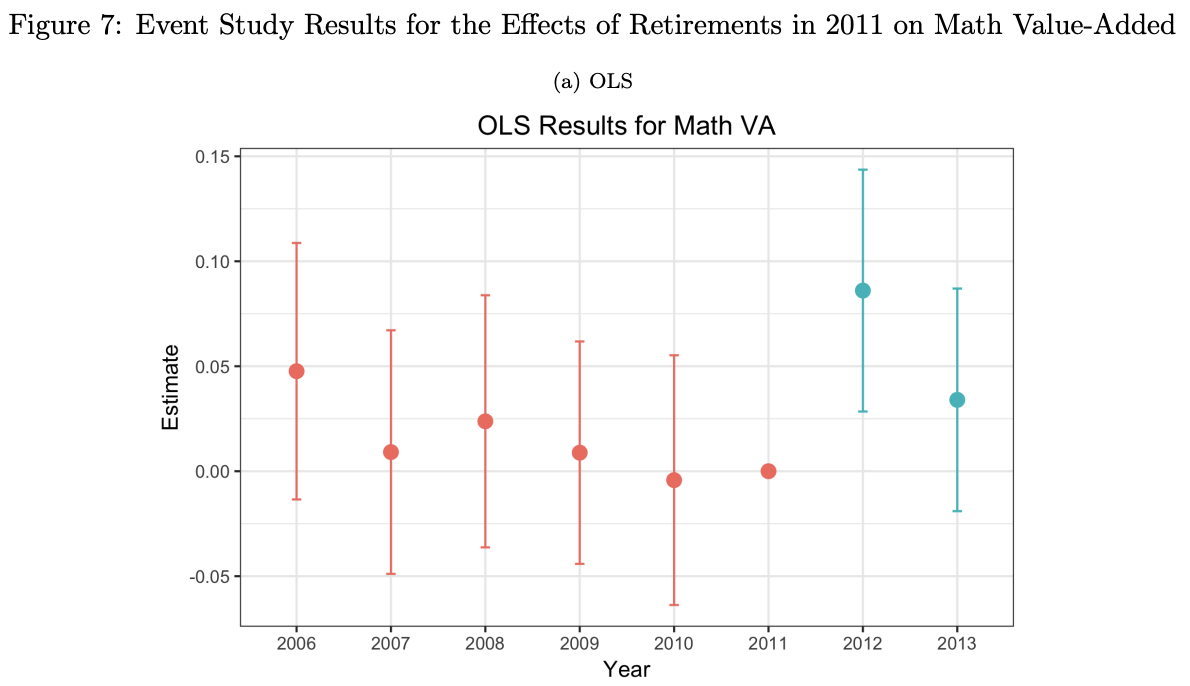
\includegraphics[width =0.75\linewidth]{Figures/act10-figure.png}
    
\end{frame}


\begin{frame}{My DiD Journey}
    \begin{wideitemize}
        \item
        I realized I had a lot of questions about the methodology of what I was doing.
            \begin{itemize}
                \item
                Should I believe parallel trends holds in this context? 
                
                \item
                Why do I have pre-trends in some of my specifications but not others? 
                
                \item
                Is it okay if I focus only on the specifications without pre-trends...? 
            \end{itemize}
        
        \pause    
        \item Pretty quickly I started writing methodological papers about these topics
            \begin{itemize}
                \item 
                I never published the Act 10 paper -- oops!
            \end{itemize}
            
        \item But the goal of my research has always been to try to inform real-world analyses of economic topics
        
        \pause
        \item Today I hope to share with you some of the insights that I and others have learned over the last few years, with the \textbf{goal of helping you improve your research.} 
            \begin{itemize}
                \item 
                Focus on both theory and applying it in practice!
            \end{itemize}
        
    \end{wideitemize}    
\end{frame}


\begin{frame}{(Approximate) Schedule for the day}
    XX
\end{frame}


\begin{frame}{Course logistics}
    \begin{wideitemize}
        \item
        I strongly encourage you all to participate and ask questions!
            \begin{itemize}
                \item 
                It's more fun for me and helps you learn better!
            \end{itemize}    
        \item
        There are several ways that you can ask questions:
        
            \begin{wideitemize}
                \item
                Raise hand on Zoom
                
                \item
                Text question on Discord
            \end{wideitemize}
            
        \item
        I will pause periodically for you to ask live questions and to review messages on Discord
    \end{wideitemize}
    
\end{frame}


\begin{frame}{Introduction}
\begin{wideitemize}
\item
\textbf{Difference-in-differences} (DiD) is one of the most popular strategies for estimating causal effects in non-experimental contexts.
\medskip
    \begin{itemize}
        \item
        Used in over 20\% of NBER WPs \citep{currie_technology_2020}
    \end{itemize}

\item
The last few years have seen an explosion of econometrics on DiD, making it hard to keep up (sorry!)

\item
In Roth, Sant'Anna, Bilinski, and Poe (RSBP 2022), we attempted to synthesize the recent literature and provide concrete recommendations for practitioners


\item
This course is loosely based on the structure in RSBP (2022), focusing on staggered timing (Section 3) and violations of parallel trends (Section 4)
\end{wideitemize}
\end{frame}


\begin{frame}{The simplest case}
\begin{wideitemize}

\item
We will start a description of DiD in the simplest ``canonical'' case

\item
Why? Because recent DiD lit can be viewed as relaxing various components of the canonical model while preserving others
\end{wideitemize}


\pause
In the canonical DiD model, we have:

\medskip 


\begin{wideitemize}
\item
2 periods: treatment occurs (for some units) in period 2

\item
Identification of the ATT from parallel trends and no anticipation

\item
Estimation using sample analogs, equivalent to OLS with TWFE

\item
A large number of independent observations (or clusters)
\end{wideitemize}    
\end{frame}


\begin{frame}{Canonical DiD -- with math}
\begin{wideitemize}
\item
Panel data on $Y_{it}$ for $t=1,2$ and $i = 1,...,N$

\item
\textbf{Treatment timing:} Some units ($D_i=1$) are treated in period $2$; everyone else is untreated $(D_i=0)$

\pause
\item
\textbf{Potential outcomes:} Observe $Y_{it}(1) \equiv Y_{it}(0,1)$ for treated units; and $Y_{it}(0) \equiv Y_{it}(0,0)$ for comparison
\end{wideitemize}    
\end{frame}

\begin{frame}{Key identifying assumptions}
\begin{wideitemize}
    \item
    \textbf{Parallel trends:} 
    \begin{equation}
\expe{ Y_{i2}(0) - Y_{i1}(0) \,|\, D_i = 1 } = \expe{ Y_{i2}(0) - Y_{i1}(0) \,|\, D_i = 0 } . \label{eqn: pt - 2 periods}
\end{equation}


    \pause
    \item
    \textbf{No anticipation:} $Y_{i1}(1) = Y_{i1}(0)$
        \begin{itemize}
            \item 
            Intuitively, outcome in period 1 isn't affected by treatment status in period 2
            
            \item
            Often left implicit in notation, but important for interpreting DiD estimand as a causal effect in period 2
        \end{itemize}
\end{wideitemize}
\end{frame}


\begin{frame}{Identification}
\begin{wideitemize}
    \item
    \textbf{Target parameter:} Average treatment effect on the treated (ATT) in period 2
    
    $$\tau_{ATT} = E[Y_{i2}(1) - Y_{i2}(0) | D_i=1] $$
    
    \pause
    \item
    Under parallel trends and no anticipation, can show that
    
    $$\tau_{ATT} = \underbrace{(E[Y_{i2} | D_i = 1] - E[Y_{i1}| D_i =1])}_{\text{Change for treated}} - \underbrace{(E[Y_{i2} | D_i = 0] - E[Y_{i1}| D_i =0]) }_{\text{Change for control}},$$
    
    \noindent a ``difference-in-differences'' of population means
\end{wideitemize}    
\end{frame}

\begin{frame}{Proof of Identification Argument}
\begin{itemize}
    \item
    Start with 
    $$E[Y_{i2}- Y_{i1}| D_i =1] - E[Y_{i2} - Y_{i1}| D_i =0]$$
    
    \pause
    \item 
    Apply definition of POs to obtain: 
    $$E[Y_{i2}(1) - Y_{i1}(1)| D_i =1] - E[Y_{i2}(0) - Y_{i1}(0)| D_i =1]$$
    
    \pause
    \item
    Use No Anticipation to substitute $Y_{i2}(0)$ for $Y_{i2}(1)$:
    $$E[Y_{i2}(1) - Y_{i1}(0)| D_i =1] - E[Y_{i2}(0) - Y_{i1}(0)| D_i =1]$$
    
    \pause
    \item
    Add and subtract $E[ Y_{i2}(0) | D_i =1] $ to obtain: 
    \begin{align*}
        &\textcolor{blue}{E[ Y_{i2}(1) - Y_{i2}(0) | D_i =1]} + \\
& \hspace{1cm} \textcolor{orange}{\left[ (E[Y_{i2}(0) | D_i = 1] - E[Y_{i1}(0)| D_i =1]) - (E[Y_{i2}(0) | D_i = 0] - E[Y_{i1}(0)| D_i =0]) \right]}
    \end{align*} 
    
    \pause
    \item
    Cancel the \textcolor{orange}{last term} using PT to get $\textcolor{blue}{E[Y_{i2}(1) - Y_{i2}(0) | D_i = 1] = \tau_{ATT}}$
\end{itemize}


\end{frame}

\begin{frame}{Estimation and Inference}
\begin{wideitemize}
    \item
    The most conceptually simple estimator replaces population means with sample analogs: 
    
    $$\hat{\tau}_{DiD} = (\bar{Y}_{12} - \bar{Y}_{11}) - (\bar{Y}_{02} - \bar{Y}_{01}) $$
    
    \noindent where $\bar{Y}_{dt}$ is sample mean for group $d$ in period $t$
    
    \pause
    \item
    Conveniently, $\hat\tau_{DID}$ is algebraically equal to OLS coefficient $\hat\beta$ from
    
\begin{equation}
    Y_{it} = \alpha_i + \phi_t + D_{it} \beta  + \epsilon_{it}, \label{eqn: TWFE-2-periods}
\end{equation}
    \noindent where $D_{it} = D_i * 1[t=2]$.
    \pause
    \item
    \textbf{Inference:} And clustered standard errors are valid as number of clusters grows large
\end{wideitemize}    
\end{frame}

\begin{frame}{Characterizing the recent literature}
We can group the recent innovations in DiD lit by which elements of the canonical model they relax:
\medskip 

\begin{wideitemize}
    \item
    \textbf{Multiple periods and staggered treatment timing}
        
    \item
    \textbf{Relaxing or allowing PT to be violated}
        
    \item
    \textbf{Inference with a small number of clusters}
    
\end{wideitemize}    
\medskip
Will focus today on the first two
\end{frame}

\backupbegin
\bibliography{Bibliography.bib}
\backupend
\end{document}